\subsection{Dataflows}
I følgende afsnit beskrives data flow fra én handling til den næste, ud fra nogle udvalgte use cases, så der kan kommer et indblik på hvornår der bliver hentet, gemt og oprettet data. Her er data flow beskrevet med aktivitetsdiagrammer \cite{gh:UMLActivityDiagrams}, hvor det data der går gennem diagrammet er beskrevet med objektnoder. Handlinger er firkanterne med runde hjørner og objektnoderne er firkanterne med skarpe hjørner.   

\subsubsection{UC1 - Kontant salg}
Et kontant salg skal både vise alle de produkter der kan købes, men også gemme salget og transaktionen efter købet er afsluttet. Dette er illustreret på \ref{fig:AD_UC1}

\begin{figure}[H]
    \centering
    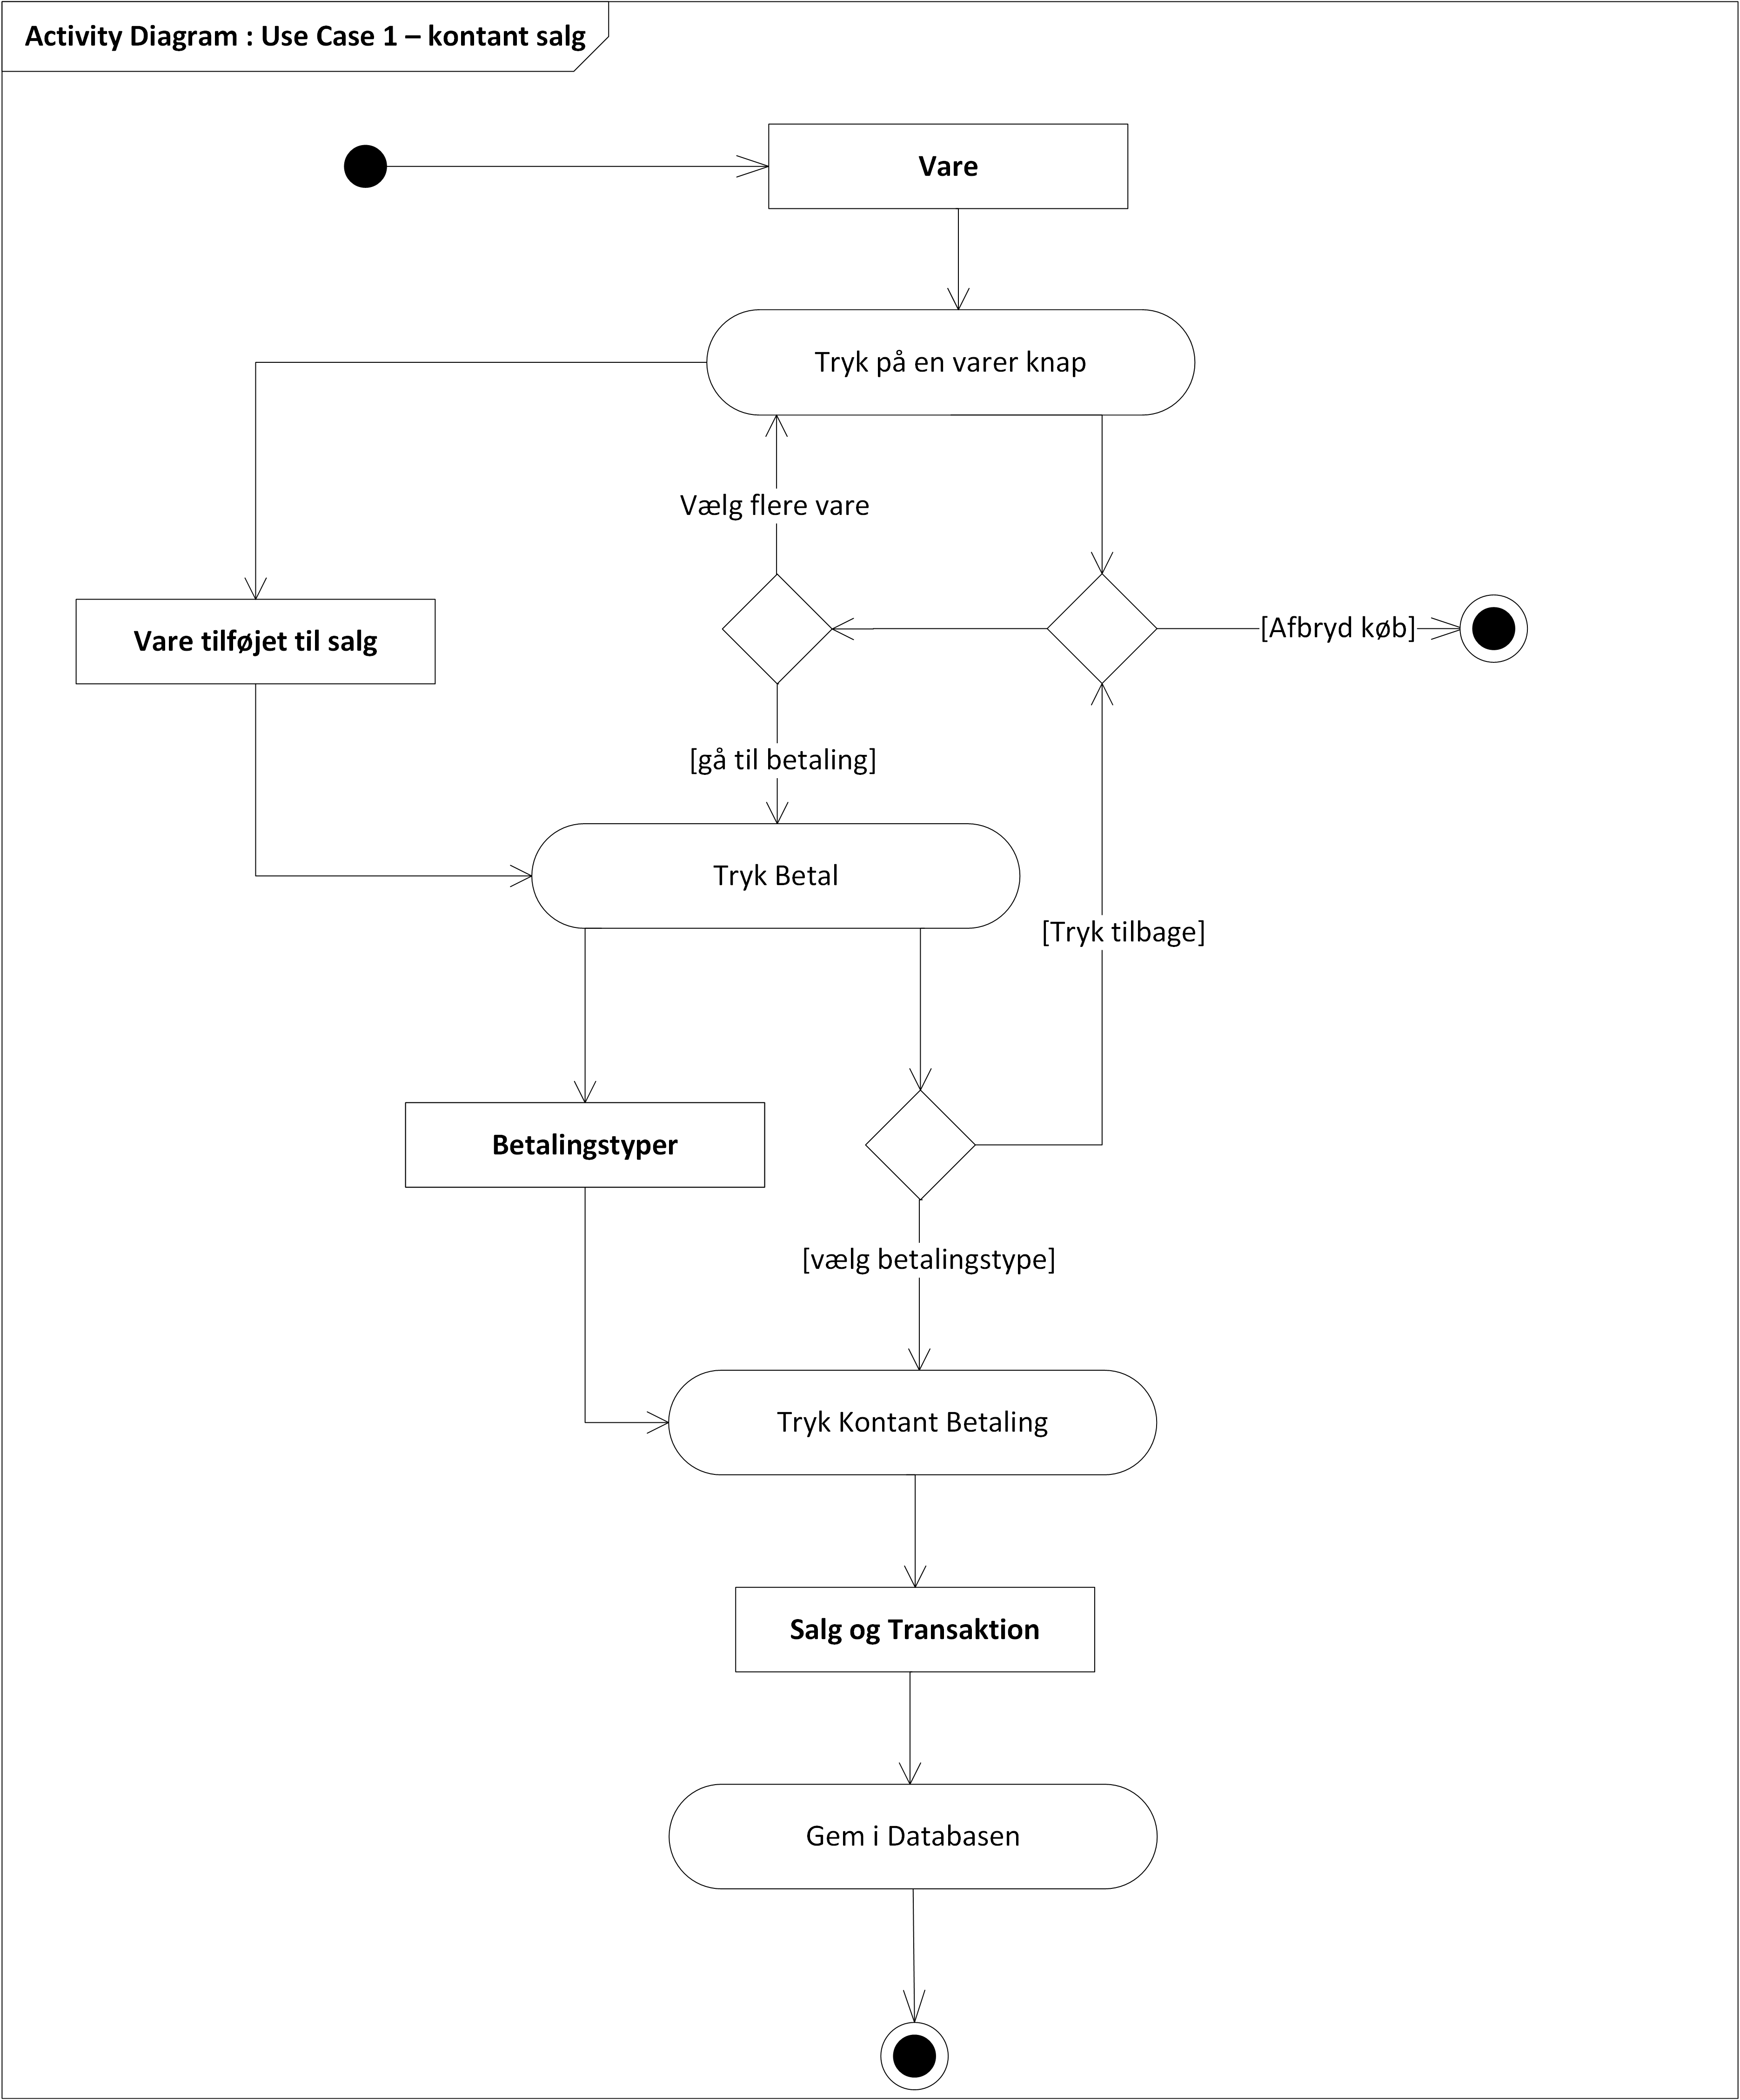
\includegraphics[width=0.8\textwidth]{N+1/DataView/DataFlow/UC1}
    \caption{Aktivitetsdiagram - Kontant salg}
    \label{fig:AD_UC1}
\end{figure}    

Varerne, som hedder Product i databasen, bliver hentet ud så de alle kan ses på GUI'en. Derefter kan man trykke på den vare man ønsker. De valgte varer bliver løbende tilføjet til salget, som i systemet er klassen \texttt{SaleOrder} der kan ses under Model pakken \ref{fig:Models_CLASS}. Når alle de ønskede varer er valgt bliver alle betalingsmuligheder vist og når kontant betaling er trykket, bliver salget og transaktionen gemt i databasen. 

\subsubsection{UC9 - Tilføj varer til kasseapparat}
For at tilføje varer, skal det være muligt at kunne se de allerede eksisterende varer og derefter gemme den vare man ønsker i databasen. Dette er illustreret på \ref{fig:AD_UC9}

\begin{figure}[H]
    \centering
    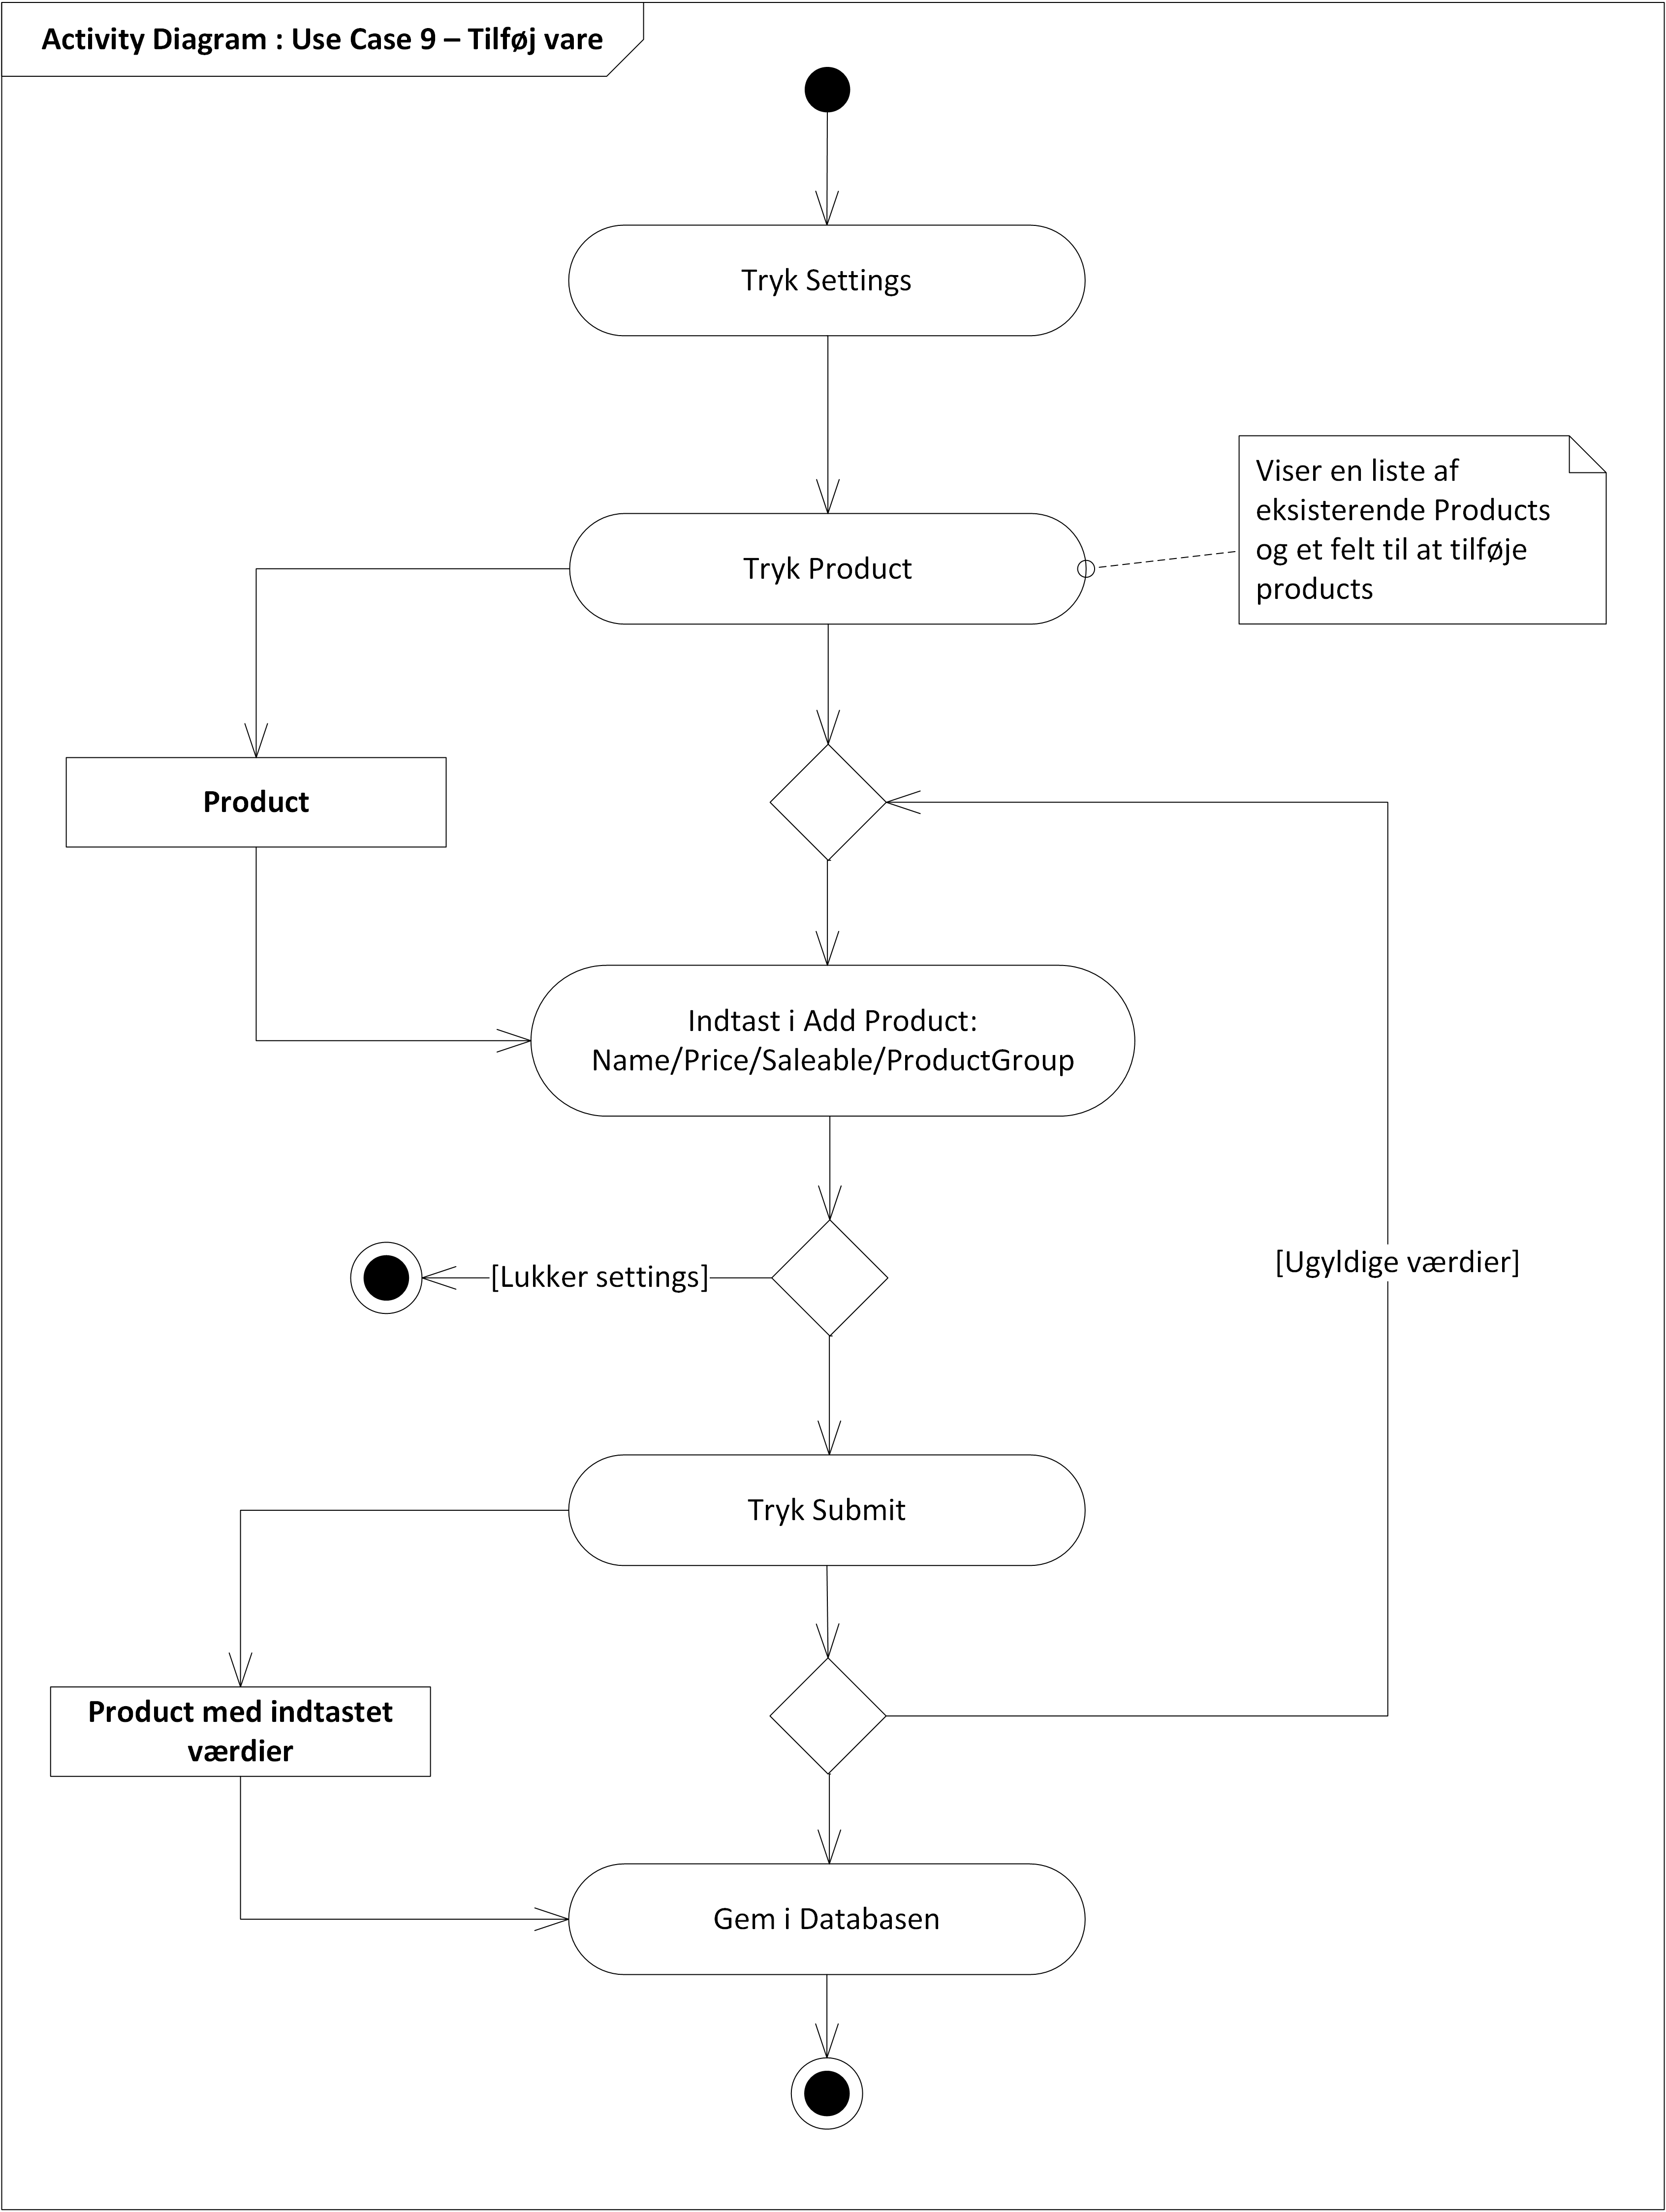
\includegraphics[width=0.8\textwidth]{N+1/DataView/DataFlow/UC9}
    \caption{Aktivitetsdiagram - Tilføj varer til kasseapparat}
    \label{fig:AD_UC9}
\end{figure}    

Varer er gemt som Products, de bliver hentet ud så det er muligt at se hvilke varer der allerede eksisterer i systemet. I feltet hvor man kan tilføje vare udfylder man alle dens værdier, hvis værdierne er gyldige bliver de gemt i databasen. 

\subsection{UC12 - Vis statistik over salg}
Det skal være muligt at se de salg der har været foretaget tidligere i systemet. Alle salg bliver løbende gemt i databasen, hvor de derefter kan ses under statestic i Web Api'et. Dette er illustreret på \ref{fig:AD_UC12}

\begin{figure}[H]
    \centering
    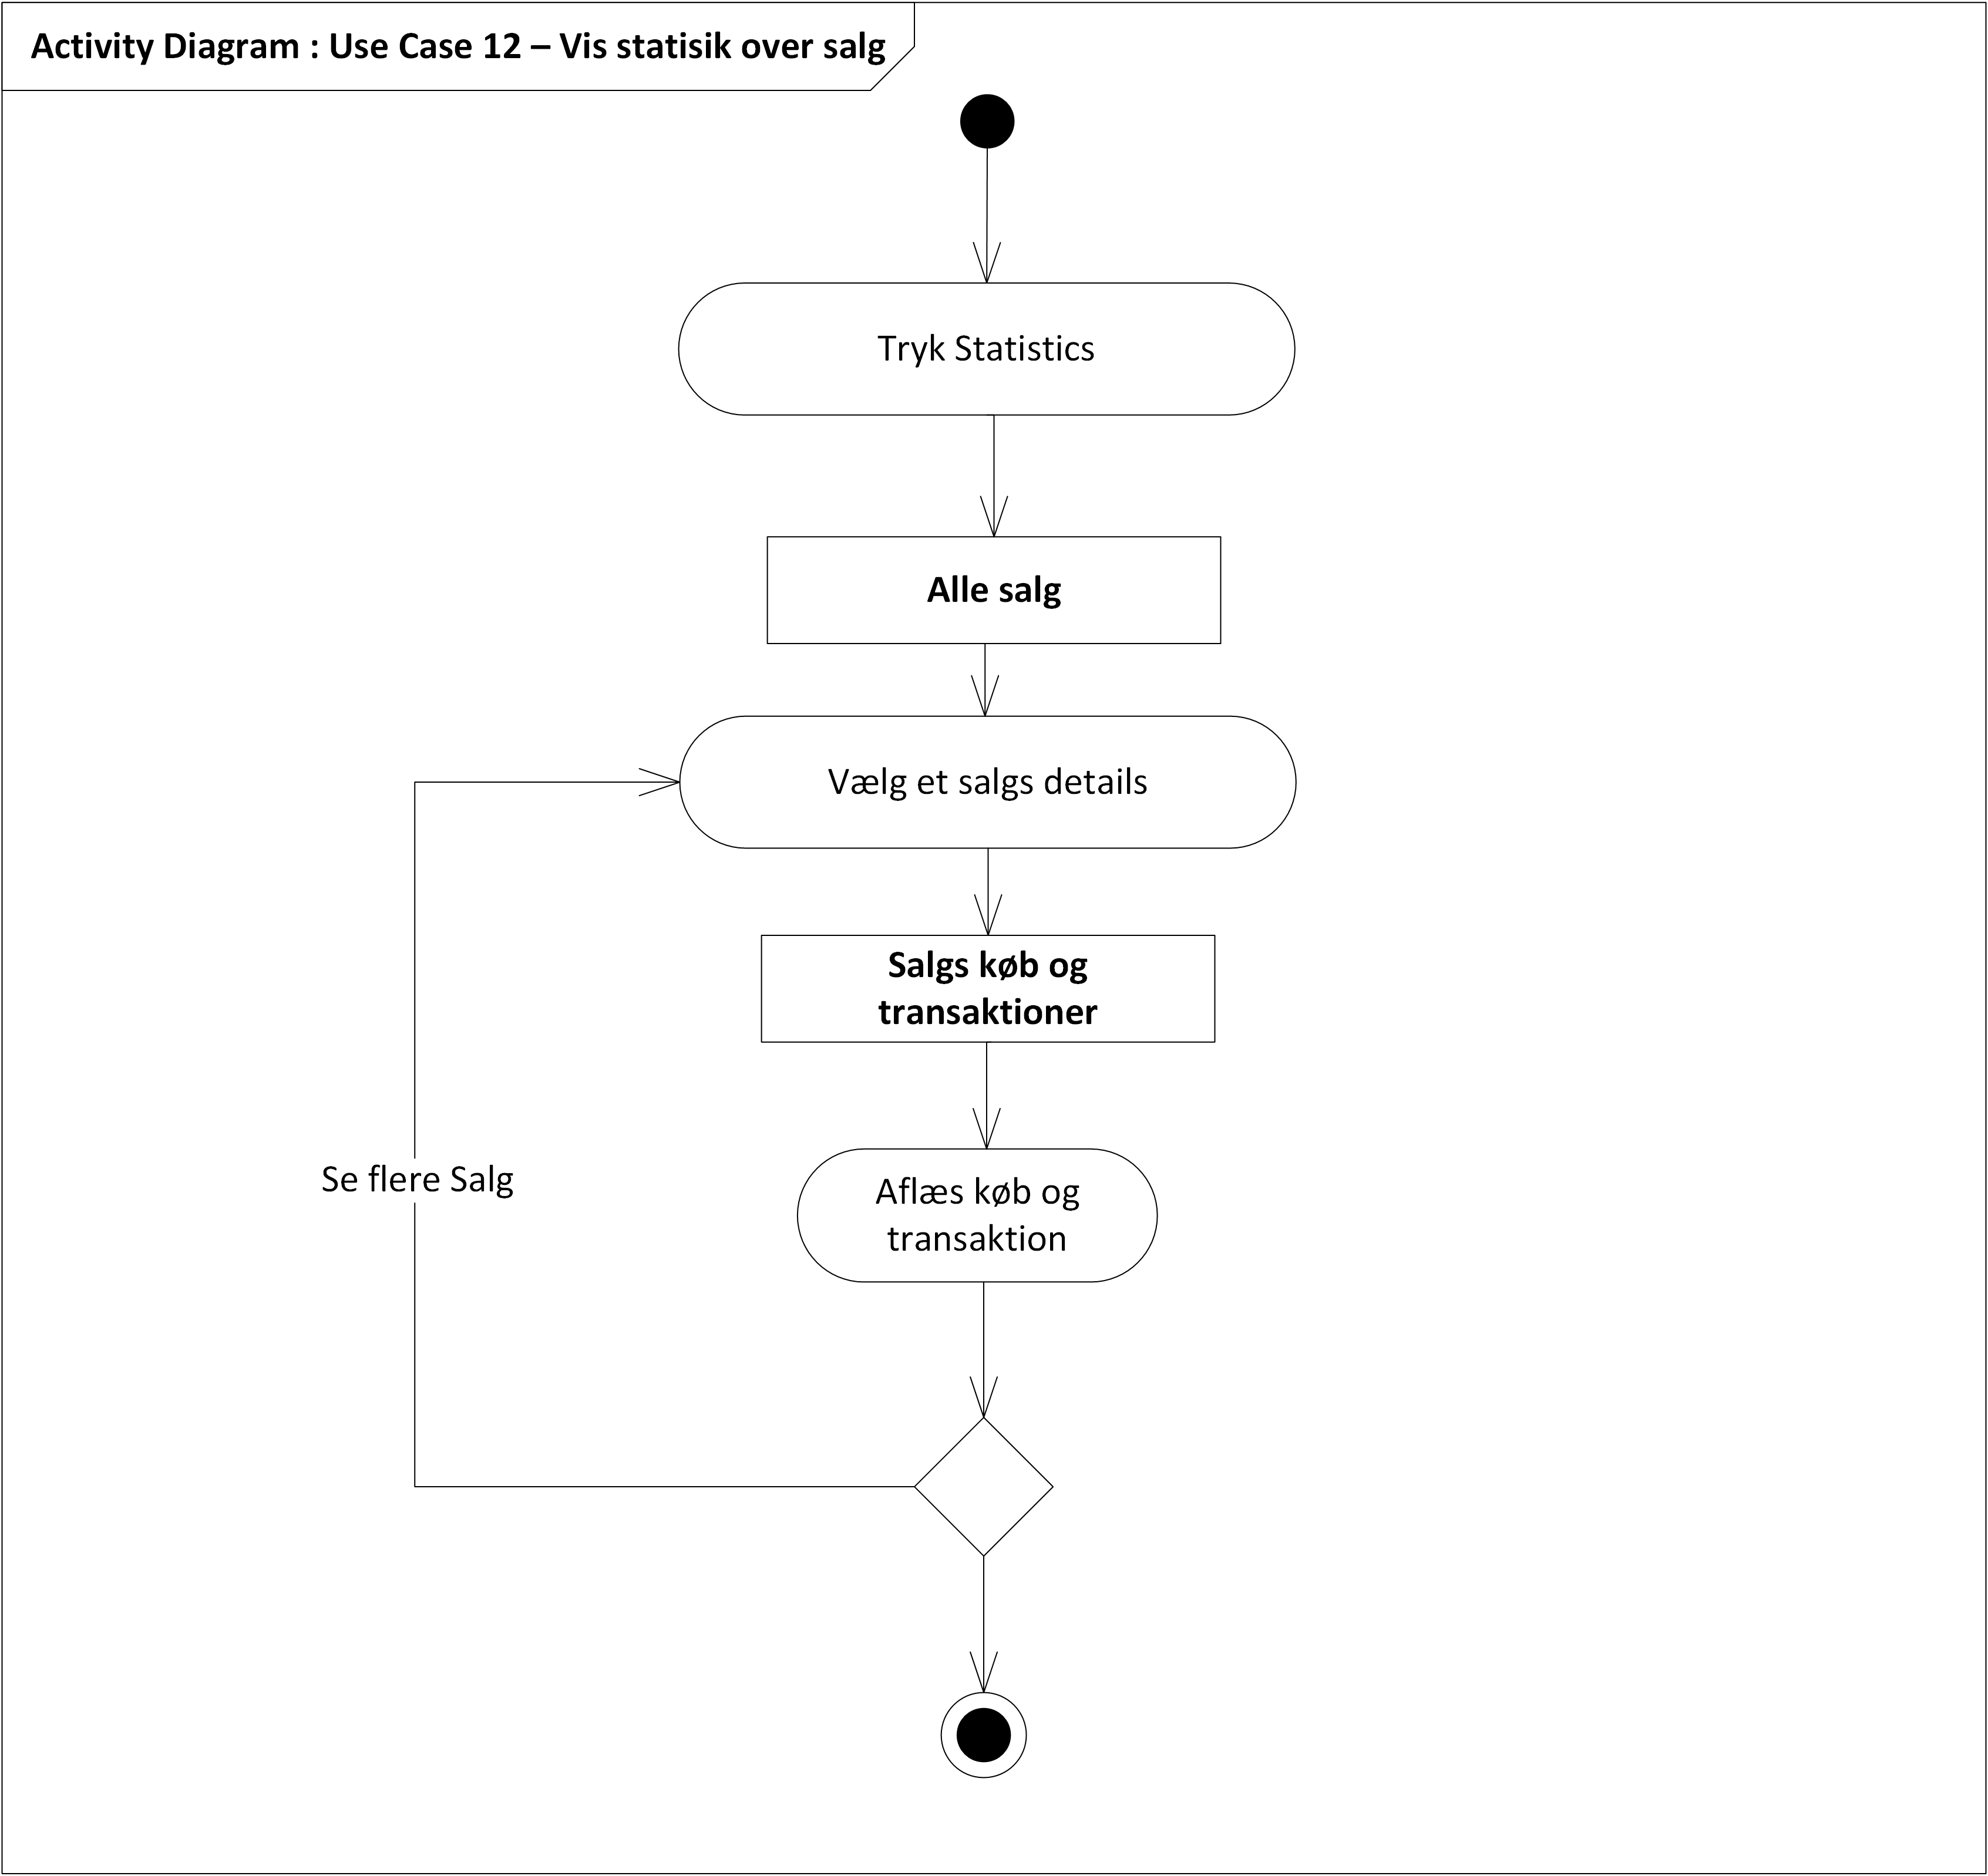
\includegraphics[width=0.8\textwidth]{N+1/DataView/DataFlow/UC12}
    \caption{Aktivitetsdiagram - Vis statistik over salg}
    \label{fig:AD_UC12}
\end{figure} 

Statistic viser en side over alle salg de salg der har været. I databasen hedder disse salg, \texttt{SalesOrder}. Her kan man gå ind under alle salg og se detaljer om de varer der er købt og hvordan transaktionerne forløb. 